\documentclass[11pt, a4paper, lithuanian]{article}

\usepackage[left=25mm,right=15mm,top=15mm,bottom=15mm]{geometry}
\usepackage[utf8x]{inputenc}
\usepackage[L7x]{fontenc}
\usepackage[lithuanian]{babel}
\usepackage{listings}
\usepackage{amsmath, amssymb}
\usepackage{graphicx}

\author{AKSfm-15, Maksim Norkin}
\title{Spindulio tipo bazinių funkcijų (angl. Radial Basis Function) tinklo mokymo algortimo įgyvendinimas}

\lstset{
  language=Matlab,
  basicstyle=\footnotesize,
  columns=fixed,
  numbers=none,
  showspaces=false,
  xleftmargin=20pt
}

\begin{document}

    \maketitle

    \section{Užduotis}

    Nenaudodami MATLAB specializuotų funkcijų (newrb, train ir pan.) sukurkite spindulio tipo bazinių funkcijų tinklą, kurio mokymui parašykite funkciją patys. Neuronų tinklas galėtų, pavyzdžiui, interpoliuoti nesudėtingą dvimatę funkciją.

    \section{Pradinės sąlygos}

    Panaudosime labai paprastą vieno sluoksnio su dviem spindulio tipo bazinių funkcijų tinklą. Kaip modelį panaudosime sinuso kreivę su moduliu tam kad sinuso kreivė užsifiksuotų teigiamų reikšmių pusėje.

    Aibių ašis sudarys iš $ X \in 2 \pi $. Numatomai, prireiks dviejų centrų, kurie yra $\frac{\pi}{2}$ ir $\frac{3\pi}{2}$, radiusą parenkame pagal \ref{formula:spindulio_skaiciavimo_formule} formuluotę.

    \begin{figure}[h]
        \centering
        \caption{Spindulio skaičiavimo formulė.}
        \label{formula:spindulio_skaiciavimo_formule}
        \begin{math}
            r = \frac{2*\pi}{\sqrt{2*2}}
        \end{math}
    \end{figure}

    Visus įverčius inicijuojame Matlab aplinkome \ref{code:pradines_salygos} pav.

    \begin{figure}[h]
      \centering
      \caption{Pradinės sąlygos.}
      \label{code:pradines_salygos}
      \begin{lstlisting}
r = 1.3;

w_1 = rand;
c_1 = max(X)/4;
r_1 = r;

w_2 = rand;
c_2 = max(X)/4*3;
r_2 = r;

w_0 = rand;
      \end{lstlisting}
    \end{figure}

    \section{Mokymas}

    Mokymui yra naudojamas LMS metodas. Pirmiausiai apskaičiuojame modelio išėjimą pagal pradines sąlygas, \ref{code:modelio_isejimo_skaiciavimas} pav.

    \begin{figure}[h]
      \centering
      \caption{Modelio išėjimo skaičiavimas.}
      \label{code:modelio_isejimo_skaiciavimas}
      \begin{lstlisting}
Y2 = [];
for j=1:size(X, 2)
    y_1 = w_1 * exp(-abs(X(j) - c_1)^2/r_1^2);
    y_2 = w_2 * exp(-abs(X(j) - c_2)^2/r_2^2);
    Y2 = [Y2 sum(y_1 + y_2) + w_0];
end
      \end{lstlisting}
    \end{figure}

    Toliau yra apskaičiuojama klaida ir pakoreguojami modelio įverčiai, \ref{code:sumines_klaidos_skaiciavimas} pav.

    \begin{figure}[h]
      \centering
      \caption{Suminės klaidos skaičiavimas ir įverčių atnaujinimas.}
      \label{code:sumines_klaidos_skaiciavimas}
      \begin{lstlisting}
Err_sum = sum(Y2 - Y);
    
w_1 = w_1 + mu * Err_sum;
w_2 = w_2 + mu * Err_sum;
w_0 = w_0 - mu * Err_sum;

Err = [Err, Err_sum];
      \end{lstlisting}
    \end{figure}

    Laukiame kuomet klaida konverguoja į nulį ir nutraukiame mokymą. 

    \section{Aproksimavimo rezultatas}

    Rezultate gauname tokį gražų grafiką, \ref{fig:aproksimavimo_rezultatas} pav.

    \begin{figure}[!ht]
      \centering
      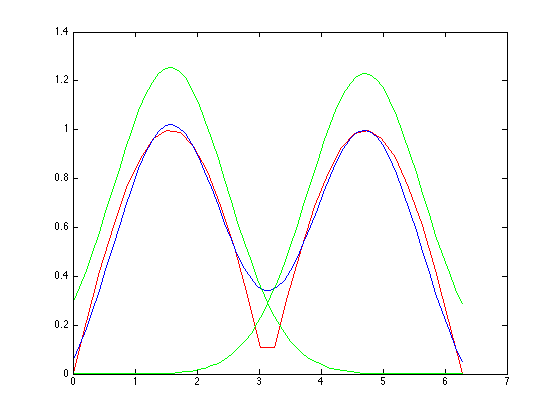
\includegraphics[width=300px]{img/rezultatas.png}
      \caption{Aproksimavimo rezultatas. Raudona linija nurodo norimą pasiekti modelio išėjimą, žalia linija parodo kiekvieno iš spindulio bazės išėjimo įtaka suminiam išėjimui. Mėlyna linija parodo viso modelio išėjimą.}
      \label{fig:aproksimavimo_rezultatas}
    \end{figure}

    \section{Išvados}

    Laboratorinio darbo metu buvo sukurtas spindulio tipo bazinių funkcijų tinklas, nenaudojant jokių Matlab specializuotų funkcijų. Neuronų tinklas interpoliuoja sinusinį virpesį. Žinant signalo charakteristikas, buvo pasirinktas dviejų perceptronų tinklas su dviem centrais ir apskaičiuotu spinduliu. Mokymas buvo atliktas naudojant LMS.

\end{document}